\documentclass[10pt,a4paper]{article}
\usepackage[margin=0.86in]{geometry}
\usepackage[T1]{fontenc}
\usepackage[utf8]{inputenc}
\usepackage{lmodern,microtype}
\usepackage{amsmath,amssymb,amsthm,mathtools}
\usepackage{booktabs,longtable,array,multicol}
\usepackage{hyperref,xcolor,graphicx,enumitem,tikz,fancyhdr}
\usetikzlibrary{positioning,arrows.meta,calc,fit}
\definecolor{navy}{HTML}{183B5A}
\definecolor{teal}{HTML}{166A76}
\definecolor{muted}{HTML}{526272}
\hypersetup{colorlinks=true,urlcolor=teal,citecolor=teal,linkcolor=navy,pdfauthor={Research working draft prepared for Mohammad Amanlou},pdftitle={REFLEX-P: Principal-Aware Robustness of Delegated AI Audits}}
\pagestyle{fancy}\fancyhf{}\fancyhead[L]{\footnotesize\textcolor{muted}{REFLEX-P | Technical research working paper}}\fancyhead[R]{\footnotesize\textcolor{muted}{22 Nov 2026}}\fancyfoot[C]{\thepage}\setlength{\headheight}{13pt}
\newtheorem{theorem}{Theorem}
\newtheorem{proposition}[theorem]{Proposition}
\newtheorem{corollary}[theorem]{Corollary}
\newtheorem{lemma}[theorem]{Lemma}
\newtheorem{observation}[theorem]{Observation}
\theoremstyle{definition}\newtheorem{definition}[theorem]{Definition}
\newcommand{\F}{\mathbb F_2}
\newcommand{\Princ}{\mathcal P}
\newcommand{\Odd}{\operatorname{Odd}}
\newcommand{\cost}{\operatorname{cost}}
\newcommand{\im}{\operatorname{im}}
\newcommand{\wt}{\operatorname{wt}}
\newcommand{\xor}{\mathbin{\oplus}}
\setlist[itemize]{leftmargin=1.35em,topsep=3pt,itemsep=2pt}
\setlist[enumerate]{leftmargin=1.35em,topsep=3pt,itemsep=2pt}
\begin{document}
\begin{center}
{\footnotesize\bfseries\textcolor{teal}{REFLEX 6.0 / RESEARCH WORKING PAPER --- NOT SUBMISSION-READY}}\\[6pt]
{\LARGE\bfseries\textcolor{navy}{Principal-Aware Robustness of\\[3pt] Delegated AI Audits}}\\[6pt]
{\large Collusion-Resilient Evidence Certification under Strategic Delegation}\\[8pt]
{\small A mathematical and computational research direction prepared for Mohammad Amanlou}\\[3pt]
{\footnotesize\textcolor{muted}{University of Tehran | Prospective multi-agent systems research | 22 November 2026}}
\end{center}
\noindent{\footnotesize\textbf{Code and reproducibility: }\url{https://github.com/MohammadAmanlou/REFLEX}}\par\vspace{4pt}
\vspace{4pt}
\noindent\colorbox{navy!6}{\parbox{0.967\linewidth}{\small\textbf{Research status and integrity note.} The structural statements below are proved for an explicit, restricted binary model and checked computationally. They have not been peer reviewed or certified as historically original. Related signed-graph, group-feedback-set, and coding results are important prior art. A general incentive-compatible mechanism, scalable synthesis method, and authentic multi-agent evaluation remain uncompleted research objectives.}}
\vspace{10pt}
\begin{abstract}
When a human principal delegates to multiple AI agents, ordinary edge-error budgets overstate independence: one colluding principal may control many delegates and corrupt every report incident to them. We study a binary, authority-labelled audit graph with arbitrary nuisance offsets and an adversary that compromises at most $k$ \emph{distinct principals}, not $k$ agent identities or individual edges. We characterize robust identifiability exactly by a principal-labelled signed-cycle transversal: $\tau_{\Princ}(G,b)>2k$. We give a constructive hypothesis feasibility decoder, a compact owner-disjoint-cycle certificate, a counterexample to edge-level robustness, monotonicity laws for safe network refinements, and a small exact audit-design solver. Our random exhaustive tests (120 small graphs), attack trials (2,000), and a 12-edge optimal-design instance pass. We distinguish these confirmed restricted-model results from the unresolved higher-value goal: synthesizing minimal-cost, \emph{incentive-compatible}, principal-aware audit institutions under dynamic delegation, uncertain evidence provenance, and adversarial equilibrium selection. The paper is a defensible technical foundation and research agenda, \emph{not} an accepted novelty claim.
\end{abstract}
\section{The technical gap---and why the previous model was insufficient}
Prior work already formalizes principal--agent delegation \cite{sourbut2024}, incentive-altering social contracts \cite{davoust2020}, optimal strategic auditing under pessimistic equilibrium selection \cite{das2026}, information acquisition from multiple agents \cite{cacciamani2024}, proof-carrying execution contracts \cite{ciliberto2026}, and corrupted group synchronization through cycle consistency \cite{lerman2021}. Signed balance and frustration, odd-cycle transversals, and group-labelled feedback sets provide mathematical tools close to ours \cite{zaslavsky2010,cygan2010,jansen2024}. Anti-collusion work in agentic AI reinforces the relevance but not the novelty of the threat model \cite{collusion2026,colosseum2026}.

The earlier REFLEX-T note assumed at most $t$ corrupted \emph{edges}. This can be profoundly misleading: three parity-sensitive, edge-disjoint cycles tolerate one arbitrary edge flip, yet a \emph{single} controlling principal incident to all three cycles can manipulate three edge reports simultaneously. The appropriate security unit is the verified \emph{ultimate principal}, with a binding map from delegates to that principal. This note derives the exact correction in a restricted model and identifies the remaining strategic implementation gap.

\section{Authority-labelled audit model}
Let $G=(V,E)$ be a finite undirected graph. Its nodes are delegated agent contexts; each edge represents a licensed, executable paired audit. A trusted registry supplies an owner map $\rho:V\to\Princ$, where $\Princ$ is the set of authentic human or institutional principals. Several vertices may share one owner; cloning an agent does not generate another principal. Let $b\in\F^E$ be an externally validated sensitivity label for each edge, and let $h\in\F$ be a binary decision-relevant state. In one episode the report on $e=uv$ is
\begin{equation}\label{eq:model}
 y_e=s_u\xor s_v\xor b_e h\xor \eta_e,\qquad s\in\F^V.
\end{equation}
The offsets $s$ can be arbitrary and mutually coordinated. For $S\subseteq\Princ$, let $V(S)=\rho^{-1}(S)$ and $\delta(S)=\{uv\in E:u\in V(S)\text{ or }v\in V(S)\}$. A Byzantine-principal attack with budget $k$ chooses some $S$ with $|S|\le k$ and any $\eta$ supported in $\delta(S)$. No independent-error assumption is made: one compromised principal may change \emph{all} incident edges. On unaffected edges, Eq.~\eqref{eq:model} is guaranteed by authenticated execution and the stipulated measurement semantics.

\textbf{Trust assumptions, not conclusions.} The model requires truthful, independently established $\rho$ and $b$, within-episode consistency of unaffected offsets, and a bound on actually compromised principals. A cryptographic signature alone does not establish that a measurement is semantically correct. Without these assumptions an agent can choose completely unconstrained $\eta$, making $h$ unidentifiable in general. Establishing credible incentives for non-Byzantine players is part of the subsequent research, not a theorem of the current model.

\begin{definition}[Principal signed-cycle transversal]\label{def:tau}
A cycle $C$ is $b$-odd if $\bigoplus_{e\in C}b_e=1$. Define
\begin{equation}\label{eq:tau}
 \tau_{\Princ}(G,b,\rho)=\min\left\{|S|:S\subseteq\Princ,\ \text{$G-V(S)$ contains no $b$-odd cycle}\right\}.
\end{equation}
\end{definition}
As a signed-graph parameter, $\tau_{\Princ}$ is close to vertex frustration/Group Feedback Vertex Set and should \emph{not} be represented as a new graph invariant absent stronger prior-art analysis.

\section{Exact robustness theorem}
\begin{theorem}[Principal-adversary identifiability frontier]\label{thm:robust}
In model \eqref{eq:model}, $h$ can be recovered uniquely from the full licensed transcript for every $s$ and every attacker controlling at most $k$ principals if and only if
\begin{equation}\boxed{\tau_{\Princ}(G,b,\rho)>2k.}\end{equation}
\end{theorem}
\begin{proof}
\emph{Sufficiency.} Suppose the same $y$ is produced by $h=0$, offsets $s_0$, and a corruption set $S_0$, and by $h=1$, offsets $s_1$, and a set $S_1$, with $|S_j|\le k$. On every edge not incident to $V(S_0\cup S_1)$, both error vectors vanish and therefore $b_e=(Ds_0)_e\xor(Ds_1)_e$, with $D$ the binary edge--vertex incidence matrix. Thus on $G-V(S_0\cup S_1)$ the vector $b$ is a vertex coboundary. Its XOR around every cycle is zero. At most $2k$ principals therefore hit every $b$-odd cycle, contradicting $\tau_{\Princ}>2k$.

\emph{Necessity.} If $\tau_{\Princ}\le2k$, choose a transversal $S$ of that size and partition it as $S=S_0\cup S_1$ with $|S_0|,|S_1|\le k$. On the remaining balanced graph, there exists an offset assignment $x\in\F^V$ with $b_e=(Dx)_e$ for every surviving edge; extend the assignment arbitrarily to deleted vertices. Hence $d=b\xor Dx$ has support only on $\delta(S_0)\cup\delta(S_1)$. Split each nonzero coordinate of $d$ between a vector $\eta_0$ supported on $\delta(S_0)$ and a vector $\eta_1$ supported on $\delta(S_1)$, so that $\eta_0\xor\eta_1=d$. Then the same transcript $y=\eta_0$ is consistent with $(h,s,\eta)=(0,0,\eta_0)$ and $(1,x,\eta_1)$. No deterministic or randomized decoder can guarantee correctness on both worlds.\end{proof}

The factor $2k$ is not a majority-voting heuristic: it follows from comparing \emph{two} possible explanations, each with its own adversarial principal set. This is a theorem about the explicit fault class, not about arbitrary equilibrium play.

\begin{corollary}[Exact consistency decoder]\label{cor:decode}
For each $h\in\F$, enumerate $S\subseteq\Princ$ with $|S|\le k$, delete edges incident to $V(S)$, and test whether $y_e\xor b_eh=s_u\xor s_v$ is consistent on the retained graph. Return the unique feasible $h$. The decoder is always correct if $\tau_{\Princ}>2k$, and can abstain when the condition fails. Using graph traversal to test balance, runtime is
\[O\!\left(2\sum_{j=0}^k\binom{|\Princ|}{j}(|V|+|E|)\right).\]
\end{corollary}
\begin{proof}For a fixed $S,h$, feasibility of offsets is exactly a signed-balance BFS constraint problem. Every true world passes for its actual compromised $S$; by Theorem~\ref{thm:robust} a false hypothesis cannot pass when $\tau_{\Princ}>2k$.\end{proof}
This is an exact but generally exponential-in-$k$ method; no polynomial-time universal solver is claimed.

\section{Why delegate counts and edge-error distances fail}
\begin{figure}[h]
\centering
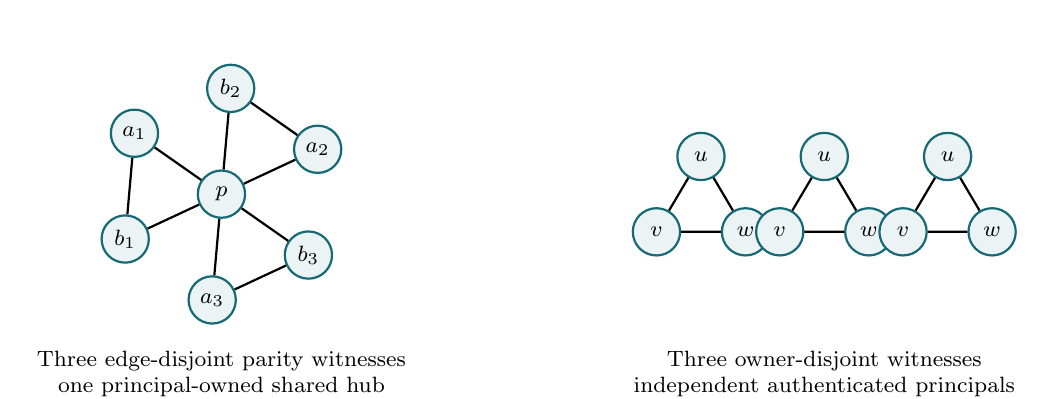
\begin{tikzpicture}[scale=.87, every node/.style={font=\footnotesize}]
\tikzstyle{agt}=[circle,draw=teal,thick,fill=teal!8,minimum size=6mm,inner sep=0pt]
\node[agt] (c) at (0,0){$p$};
\foreach \a/\b/\t in {145/205/1,25/85/2,265/325/3}{
  \node[agt] (x\t) at (\a:1.55){$a_{\t}$};
  \node[agt] (y\t) at (\b:1.55){$b_{\t}$};
  \draw[thick] (c)--(x\t)--(y\t)--(c);
}
\node[align=center,anchor=north] at (0,-2.15){Three edge-disjoint parity witnesses\\one principal-owned shared hub};
\begin{scope}[xshift=7cm]
\foreach \j in {0,1,2}{
 \begin{scope}[xshift={1.8*\j cm}]
 \node[agt] (u\j) at (0,0.55){$u$};\node[agt] (v\j) at (-.65,-.55){$v$};\node[agt] (w\j) at (.65,-.55){$w$};
 \draw[thick] (u\j)--(v\j)--(w\j)--(u\j);
 \end{scope}}
 \node[align=center,anchor=north] at (1.8,-2.15){Three owner-disjoint witnesses\\independent authenticated principals};
\end{scope}
\end{tikzpicture}
\caption{Edge-disjoint cycles are not necessarily principal-disjoint. A shared owner can corrupt all incident reports; replacing that ownership structure with genuinely independent principals changes the correct robustness threshold. Edges carry a $b$-odd sensitivity assignment (one marked edge per triangle in experiments).}\label{fig:two}
\end{figure}

Consider three $b$-odd triangles sharing a central vertex and otherwise disjoint. Their edge-error coset distance is $d_*=3$, so the old REFLEX-T bound would certify tolerance of one arbitrary \emph{edge} flip. Yet deleting the owner of the shared hub destroys all three $b$-odd cycles, yielding $\tau_{\Princ}=1$ and no guarantee against one Byzantine principal. By contrast, three vertex-disjoint $b$-odd triangles with nine genuinely independent owners have $\tau_{\Princ}=3$ and tolerate one Byzantine principal. If those nine delegates secretly belong to \emph{one} ultimate principal, $\tau_{\Princ}$ falls to $1$ despite the unchanged visible graph. The test script reproduces all three cases.

\begin{proposition}[Principal-disjoint-cycle certificate]\label{prop:packing}
If $G$ contains $2k+1$ $b$-odd cycles whose sets of \emph{principal owners} are pairwise disjoint, majority voting over their cycle parities correctly recovers $h$ under any $k$ Byzantine principals.
\end{proposition}
\begin{proof}For every cycle whose owners are uncompromised, every incident edge is uncorrupted and the XOR of its vertex offsets cancels, so its parity vote equals $h$. At most $k$ owner-disjoint cycles can intersect the $k$ compromised principals. Hence a strict majority of $2k+1$ votes is correct.\end{proof}
The packing condition is sufficient, not necessary, and finding principal-disjoint cycles can be computationally expensive. The exact transversal condition in Theorem~\ref{thm:robust} remains the completeness standard.

\section{Safe structural refinements and a sharp limitation}
\begin{proposition}[Monotonicity and identity coarsening]\label{prop:mono}
Fix authenticated principal labels and edge sensitivities. Adding authorized audit edges without removing old ones cannot decrease $\tau_{\Princ}$. Merging two authenticated owners into one ownership group, without changing the graph, cannot increase $\tau_{\Princ}$. Removing edges can decrease $\tau_{\Princ}$.
\end{proposition}
\begin{proof}Any principal set that kills every odd cycle after edge addition also killed all old cycles, hence the minimum transversal size cannot fall. For ownership merging, map any old transversal $S$ to its coarsened image; this image has no more labels and deletes at least the same vertices, so it remains a transversal. Edge removal deletes potential witnesses, which can reduce the minimum transversal.\end{proof}

Thus a system may reuse an existing sound certificate after a verified append-only audit expansion, while authority mergers, removals, or new trust assumptions require rechecking. This is a restricted, provable compositional rule; general sound incremental proof-carrying delegation is still open. \textbf{Identity authentication is essential.} The same visible reports and graph can correspond to different genuine owner maps; without a trusted owner registry, no transcript-only method can validly infer owner-level Byzantine tolerance for all possible hidden partitions.

\paragraph{Unequal compromise costs.} If principal $p$ has attacker cost $w_p>0$ and each world has budget $B$, the exact condition is: \emph{for every pair} $S_0,S_1$ with $w(S_j)\le B$, $G-V(S_0\cup S_1)$ retains a $b$-odd cycle. The tempting scalar rule $\min_S w(S)>2B$ is sufficient but \emph{not necessary} when weights cannot be partitioned between two budget-feasible adversaries. This detail matters for realistic institution-level threat models.

\section{Minimum-cost licensed audit design}
Let $E_{\rm cand}$ be candidate licensed measurements, each with verified positive cost $c_e$. For a selected audit subgraph $F\subseteq E_{\rm cand}$, define
\begin{equation}\label{eq:design}
 \min_{F\subseteq E_{\rm cand}}\sum_{e\in F}c_e\quad\text{s.t.}\quad\tau_{\Princ}(V,F,b|_F,\rho)>2k.
\end{equation}
The preceding theorem gives an exact certification oracle. A complete small-instance algorithm enumerates subsets $F$, rejects those with non-increasing costs, and checks the robustness condition by enumerating principal deletion sets of size at most $2k$. Its bound is exponential in $|E_{\rm cand}|$; this note makes no claim of scalable optimal synthesis.

\textbf{Candidate scalable research direction.} Counterexample-guided synthesis would alternate between (i) selecting a low-cost audited edge set and (ii) an adversary oracle returning $\le2k$ principals whose deletion makes the chosen signed graph balanced. Each such witness imposes a new requirement for at least one licensed $b$-odd cycle outside the returned owners. Efficient separation, approximation, structural parameters, and dynamic certificate reuse constitute the algorithmic challenge. This approach draws on standard cutting-plane and CEGIS ideas; novelty must come from new guarantees for the specific \emph{strategic} problem, not naming the loop.

\section{Strategic implementability is not obtained for free}
The present proofs make an important epistemic promise only \emph{conditional on the protocol correctness of noncompromised reports}. They do not enforce that premise. A rigorous principal--agent extension needs a game with explicit payoffs, action capabilities, entry and exit, side payments, equilibrium selection, and coalition deviations.

\begin{observation}[No unrestricted-report guarantee]\label{obs:no}
If every principal may change arbitrary incident report bits without a binding constraint, an audit transcript does not identify $h$ in general, regardless of the number of cycles. In particular, choosing $\eta=bh$ makes $y=Ds$ under both states.
\end{observation}
This simple impossibility shows why assuming bounded Byzantine owners without a causal enforcement story is not an end-to-end result. One way to close the gap is an independently valid measurement oracle with enforceable deposits or payoffs; but such an oracle is itself a strong and potentially costly trust assumption. A proof-checking runtime can enforce an explicit tool contract \cite{ciliberto2026}, yet contract enforcement alone does not prove the physical truth of the reported evidence. An economic mechanism must also distinguish individually truthful behavior from coalition-profitability with transferable side payments.

\textbf{Research target 1---coalition-proof enforceability.} For every coalition $C$ of strategic (non-Byzantine) principals and every feasible joint reporting deviation $d_C$, define a genuine coalition gain $G_C(d_C)$ and an independently verifiable expected penalty $L_C(d_C;\mathcal M)$. Characterize a nontrivial mechanism family for which $L_C(d_C;\mathcal M)>G_C(d_C)$ on every harmful deviation, \emph{without} assuming the verifier already knows $h$. The last qualification is essential: an oracle that directly reveals the unknown state trivializes evidence acquisition.

\textbf{Research target 2---multi-principal governance.} A robust certificate should be tied to human/principal identity, formal authorization, and an accountable mapping of delegates to principals. Characterize which agent splitting, merging, and reassignment operations preserve a valid certificate, and when extra independent evidence must be acquired.

\textbf{Research target 3---statistical and semantic generalization.} Extend the binary test to noisy, correlated, context-dependent signals, using time-uniform confidence sequences where available. Confirm that the underlying claims, audit sensitivities, and source provenance remain valid. Human preference dynamics and distribution shift must be modeled separately; graph redundancy cannot cure false semantics.

\section{Reproducible computational checks}
The accompanying dependency-free file \texttt{reflex6\_principal\_robustness.py} implements signed balance testing, principal-transversal enumeration, a robust hypothesis feasibility decoder, exhaustive transcript enumeration, and exhaustive audit-design optimization.
\begin{center}\small
\begin{tabular}{p{.41\linewidth}p{.14\linewidth}p{.33\linewidth}}\toprule
Test & Result & Interpretation\\\midrule
120 random graphs ($3$--$5$ nodes) & 120 pass & Exhaustive transcript overlap matches $\tau_{\Princ}>2k$\\
2000 synthetic Byzantine trials & 2000 pass & Decoder returns true state under one corrupted authentic principal\\
Three hub-sharing odd triangles & $d_*=3$, $\tau=1$ & Edge-error tolerance overstates owner-level robustness\\
Three owner-disjoint odd triangles & $\tau=3$ & One corrupt principal is recoverable\\
Same nine nodes, one real owner & $\tau=1$ & Sybil identities do not create authentic principals\\
Four disjoint candidate triangles & cost $21$ & Exact 12-edge search selects three cheapest robust components\\\bottomrule
\end{tabular}
\end{center}
\noindent\textbf{Interpretation.} These are deterministic mathematical sanity checks, not experiments with deployed AI agents or results relative to state-of-the-art strategic-audit baselines. There is no claim of empirical utility or conference readiness. Future studies require both controlled strategic players (with explicit incentives and collusive behavior) and LLM-agent stress tests on reproducible tasks; only the former can validate equilibrium guarantees.

\section{Related-work map and proposed publication path}
\small
\begin{longtable}{p{.23\linewidth}p{.32\linewidth}p{.39\linewidth}}
\toprule\textbf{Source family} & \textbf{Established contribution} & \textbf{What REFLEX-P must add to become an original paper}\\\midrule\endfirsthead
\toprule\textbf{Source family} & \textbf{Established contribution} & \textbf{What remains}\\\midrule\endhead
Delegation games \cite{sourbut2024} & Principal welfare, coordination and control & Formal owner-labelled deviations, robust outcome certificates, new mechanism characterization\\
Social contracts \cite{davoust2020} & Incentive design in noncooperative games & Coalition-proof audit rights under evolving delegated authority\\
Optimal audits \cite{das2026} & Policies against strategic agents and worst-case equilibrium & Proof that a new identity-structured problem escapes their assumptions, then stronger algorithmic results\\
Information acquisition \cite{cacciamani2024} & Information gathering by several self-interested agents & Evidence semantics conditional on verified multi-principal topology, not only reports and effort\\
Proof-carrying contracts \cite{ciliberto2026} & Safety of contractual actions under delegation & Semantically grounded evidence and owner-level strategic guarantees beyond runtime safety\\
Signed graphs, GFVS \cite{zaslavsky2010,cygan2010,jansen2024} & Balance, odd-cycle transversals and parameterized algorithms & Nontrivial new complexity or constructive results beyond relabelling these classic problems\\
Robust synchronization \cite{lerman2021} & Corruption recovery from cycle consistency & Identity-aware, multi-principal strategic observation and mechanism synthesis\\
AI collusion \cite{colosseum2026,collusion2026} & Empirical collusion audits, governance risks & Formal certified intervention policies tested in game models and agent systems\\\bottomrule
\end{longtable}\normalsize

A plausible \textbf{AAMAS/IJCAI} paper should concentrate on one theorem-level contribution to coalition-proof principal-aware audit design, an algorithm with provable approximation or parameterized runtime, and calibrated comparisons against audit optimization, group-synchronization, and signed-graph baselines. General claims about NeurIPS/ICML require independently significant machine-learning theory or evidence, not merely applying LLMs to a graph theorem. The research also aligns with Rovatsos's focus on multi-agent interaction rules and incentives \cite{rovatsosprofile}, but no supervisor endorsement, PhD admission, or funding can be inferred.

\paragraph{Four-stage PhD research roadmap (proposed, not completed).}
\begin{enumerate}
\item \textbf{Year 1:} Fully specify multi-principal reporting games, audit observables, identity assumptions and two-sided impossibility results. Compare owner-labelled robustness to signed graph and coalition-verification theorems.
\item \textbf{Year 2:} Establish a mechanism-implementation theorem under explicit liability, participation and side-payment constraints; derive real complexity boundaries for contract synthesis.
\item \textbf{Year 3:} Build an incremental verifier and a solver with certified bounds; test larger synthetic games and distribution shifts; publish code and falsification tests.
\item \textbf{Year 4:} Extend to dynamic delegation and multi-criterion human preferences; validate with agentic execution under bounded misreporting and substantive independent audits.
\end{enumerate}

\paragraph{Pre-submission blocking checklist.} Before claiming a top-conference paper: (i) adversarial peer-level prior-art comparison of the \emph{new} theorem; (ii) formally proved implementation of strategically truthful reporting for a nontrivial multi-principal game; (iii) a new scalable algorithm with tight or informative bounds; (iv) meaningful empirical comparisons, error bars, ablations, and reproducibility artifacts; (v) independent mathematical review. None of these can be replaced with manuscript length or model-brand names.

\section{Conclusion}
The revision fixes a clear security modeling error: robustness must be measured at the level of independently compromised principals rather than edges or spawned delegates. The exact criterion $\tau_{\Princ}>2k$, its sound decoder, owner-disjoint certificate, and computational sanity checks provide a correct restricted-model platform. Yet most graph-theoretic ingredients have identifiable predecessors. The next candidate for a distinctive scientific contribution is a \emph{coalition-proof implementation theorem and synthesis algorithm} in which auditable evidence rights, real principal identity, and equilibrium behavior are jointly specified. Until such a result is completed, this manuscript remains a rigorous exploratory research document, not a submission-ready publication.

\small
\begin{thebibliography}{99}
\bibitem{davoust2020} A. Davoust and M. Rovatsos, ``Social Contracts for Non-Cooperative Games,'' \emph{AAAI/ACM AIES}, 2020. \url{https://www.research.ed.ac.uk/en/publications/social-contracts-for-non-cooperative-games/}.
\bibitem{sourbut2024} O. Sourbut, L. Hammond, H. Wood, ``Cooperation and Control in Delegation Games,'' \emph{IJCAI}, 2024. \url{https://www.ijcai.org/proceedings/2024/26}.
\bibitem{das2026} S. Das, F.-Y. Yu, Y. Zhang, ``Optimally Auditing Adversarial Agents,'' \emph{AAAI}, 2026. \url{https://ojs.aaai.org/index.php/AAAI/article/download/38722/42684}.
\bibitem{cacciamani2024} F. Cacciamani, F. Castiglioni, N. Gatti, ``Online Information Acquisition: Hiring Multiple Agents,'' \emph{ICLR}, 2024. \url{https://proceedings.iclr.cc/paper_files/paper/2024/hash/6358cd0cd6607fdf4870595795eb1710-Abstract-Conference.html}.
\bibitem{ciliberto2026} C. Ciliberto, A. Rudi, E. Tassi, ``Proof-Carrying Contracts: Commitments AI Agents Cannot Break,'' arXiv:2610.28484, 2026. \url{https://arxiv.org/abs/2610.28484}.
\bibitem{lerman2021} G. Lerman, Y. Shi, ``Robust Group Synchronization via Cycle-Edge Message Passing,'' \emph{Foundations of Computational Mathematics}, 2021. \url{https://link.springer.com/article/10.1007/s10208-021-09532-w}.
\bibitem{zaslavsky2010} T. Zaslavsky, ``Balance and Clustering in Signed Graphs,'' 2010. \url{https://www.researchgate.net/publication/267375644_Balance_and_Clustering_in_Signed_Graphs}.
\bibitem{cygan2010} S. Guillemot, ``FPT algorithms for path-transversal and cycle-transversal problems,'' \emph{Discrete Optimization}, 2010. \url{https://doi.org/10.1016/j.disopt.2010.05.003}.
\bibitem{jansen2024} B. M. P. Jansen et al., ``Preprocessing to Reduce the Search Space for Odd Cycle Transversal,'' \emph{IPEC}, 2024. \url{https://drops.dagstuhl.de/entities/document/10.4230/LIPIcs.IPEC.2024.15}.
\bibitem{colosseum2026} M. Nakamura et al., ``Colosseum: Auditing Collusion in Cooperative Multi-Agent Systems,'' arXiv:2602.15198, 2026. \url{https://arxiv.org/abs/2602.15198}.
\bibitem{collusion2026} ``Mapping Human Anti-Collusion Mechanisms to Multi-Agent AI Systems,'' \emph{Knowledge-Based Systems}, 2026. \url{https://www.sciencedirect.com/science/article/pii/S0950705126007938}.
\bibitem{rovatsosprofile} M. Rovatsos, \emph{University of Edinburgh academic profile}, updated 2026. \url{https://edwebprofiles.ed.ac.uk/profile/prof-michael-rovatsos}.
\bibitem{contracts2026} ``Multi-agent contract design with a budget,'' \emph{Games and Economic Behavior}, 2026. \url{https://www.sciencedirect.com/science/article/pii/S0899825626001351}.
\bibitem{evidence2026} ``Robust implementation with peer mechanisms and evidence,'' \emph{Games and Economic Behavior}, 2026. \url{https://ideas.repec.org/a/eee/gamebe/v155y2026icp192-211.html}.
\bibitem{ijcai2026} N. K. Sreenivas, K. Larson, ``Information and Contract Design for Repeated Interactions Between Agents with Misaligned Incentives,'' \emph{IJCAI}, 2026. \url{https://ijcai.org/proceedings/2026/41}.
\end{thebibliography}
\end{document}
